\documentclass[aspectratio=169,xcolor=dvipsnames]{beamer}
\usetheme{Madrid}\usecolortheme{seahorse}
\usepackage{amsmath,amssymb,listings,tikz,booktabs,hyperref}
\usetikzlibrary{arrows.meta,positioning,shapes}
\lstset{language=Python,basicstyle=\small\ttfamily,keywordstyle=\color{blue}\bfseries,
  commentstyle=\color{OliveGreen},stringstyle=\color{red},frame=single,breaklines=true}

\title[Algorithms -- Week 3]{\textbf{Thiết kế và Phân tích Thuật toán}\\
  \large Week 3: Divide and Conquer I}
\subtitle{Merge Sort, Quick Sort & Recursion \\ TOAE209/TOAH209 -- Foreign Trade University}
\author{Department of Technology \& Data Science}
\date{Semester 2024--2025}
\AtBeginSection[]{\begin{frame}<beamer>{Outline}\tableofcontents[currentsection]\end{frame}}

\begin{document}
\begin{frame}\titlepage\end{frame}
\begin{frame}{Outline}\tableofcontents\end{frame}

\section{Motivation}
\begin{frame}{The Power of Divide and Conquer}
  \begin{columns}
    \column{0.55\textwidth}
    \begin{block}{Key Idea}
      Break a problem into \textbf{smaller subproblems} of the same type,\\
      solve them recursively, then \textbf{combine} the results.
    \end{block}
    \begin{itemize}
      \item Merge Sort: $\Theta(n\log n)$ -- beats $\Theta(n^2)$ sorts
      \item Binary Search: $\Theta(\log n)$ -- beats $\Theta(n)$ scan
      \item Strassen: $\Theta(n^{2.807})$ -- beats $\Theta(n^3)$ matrix mult
      \item Karatsuba: $\Theta(n^{1.585})$ -- faster integer multiplication
    \end{itemize}
    \column{0.4\textwidth}
    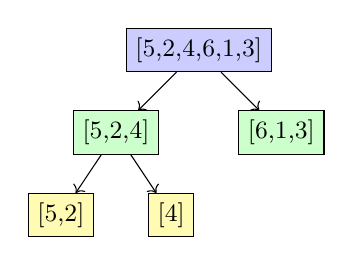
\begin{tikzpicture}[scale=0.7,font=\small]
      \node[draw,fill=blue!20] (root) at (2,4) {[5,2,4,6,1,3]};
      \node[draw,fill=green!20] (L) at (0.5,2.5) {[5,2,4]};
      \node[draw,fill=green!20] (R) at (3.5,2.5) {[6,1,3]};
      \node[draw,fill=yellow!30] (LL) at (-0.5,1) {[5,2]};
      \node[draw,fill=yellow!30] (LR) at (1.5,1) {[4]};
      \draw[->] (root)--(L); \draw[->] (root)--(R);
      \draw[->] (L)--(LL); \draw[->] (L)--(LR);
    \end{tikzpicture}
  \end{columns}
\end{frame}

\section{Historical Context}
\begin{frame}{Historical Development}
  \begin{description}
    \item[1945] John von Neumann invents Merge Sort
    \item[1959] Tony Hoare invents Quicksort (``the most elegant algorithm ever written'')
    \item[1960s] Divide and conquer formalised as a design paradigm
    \item[1969] Strassen's sub-cubic matrix multiplication
    \item[1971] Knuth analyses Quicksort rigorously in TAOCP
    \item[1980s] D\&C becomes standard in algorithm design textbooks
    \item[2018] Tim Peters' Timsort (hybrid merge+insertion) used in Python, Java
  \end{description}
\end{frame}

\section{Merge Sort}
\begin{frame}[fragile]{Merge Sort: Design}
  \textbf{Three steps:} Divide, Conquer, Combine
  \begin{lstlisting}
def merge_sort(arr):
    if len(arr) <= 1:
        return arr                   # Base case
    mid = len(arr) // 2
    L = merge_sort(arr[:mid])        # Conquer left
    R = merge_sort(arr[mid:])        # Conquer right
    return merge(L, R)               # Combine

def merge(L, R):
    result, i, j = [], 0, 0
    while i < len(L) and j < len(R):
        if L[i] <= R[j]:             # Stability: <=
            result.append(L[i]); i += 1
        else:
            result.append(R[j]); j += 1
    return result + L[i:] + R[j:]
  \end{lstlisting}
\end{frame}

\begin{frame}{Merge Sort: Analysis}
  \textbf{Recurrence:} $T(n) = 2T(n/2) + \Theta(n)$\\[6pt]
  \textbf{Recursion Tree:}
  \begin{itemize}
    \item Level 0: $cn$ work, 1 node
    \item Level 1: $cn/2 + cn/2 = cn$ work, 2 nodes
    \item Level $k$: $cn$ work, $2^k$ nodes
    \item Total levels: $\log_2 n$
  \end{itemize}
  \textbf{Total work:} $cn \times \log_2 n = \Theta(n\log n)$\\[6pt]
  \begin{block}{Properties}
    \begin{itemize}
      \item Time: $\Theta(n\log n)$ worst/average/best
      \item Space: $\Theta(n)$ auxiliary (NOT in-place)
      \item Stable: yes (preserves relative order of equal elements)
    \end{itemize}
  \end{block}
\end{frame}

\section{Quick Sort}
\begin{frame}[fragile]{Quick Sort: Lomuto Partition}
  \begin{lstlisting}
def partition(arr, lo, hi):
    pivot = arr[hi]          # choose last element as pivot
    i = lo - 1
    for j in range(lo, hi):
        if arr[j] <= pivot:
            i += 1
            arr[i], arr[j] = arr[j], arr[i]
    arr[i+1], arr[hi] = arr[hi], arr[i+1]
    return i + 1             # pivot's final position

def quicksort(arr, lo=0, hi=None):
    if hi is None: hi = len(arr) - 1
    if lo < hi:
        p = partition(arr, lo, hi)
        quicksort(arr, lo, p - 1)
        quicksort(arr, p + 1, hi)
  \end{lstlisting}
\end{frame}

\begin{frame}{Quick Sort: Analysis}
  \begin{columns}
    \column{0.45\textwidth}
    \begin{alertblock}{Worst Case $\Theta(n^2)$}
      Pivot is always min or max.\\
      Happens with already-sorted input + last-element pivot.\\
      $T(n) = T(n-1) + \Theta(n)$
    \end{alertblock}
    \column{0.45\textwidth}
    \begin{exampleblock}{Average Case $\Theta(n\log n)$}
      Expected over random permutations.\\
      Each element is compared $O(\log n)$ times on average.\\
      With \textbf{random pivot}: worst case with prob $\to 0$.
    \end{exampleblock}
  \end{columns}
  \vspace{0.5em}
  \textbf{Properties:}
  \begin{itemize}
    \item In-place: $\Theta(1)$ extra space (ignoring stack)
    \item NOT stable (Lomuto partition)
    \item Cache-friendly: good locality of reference
    \item In practice, often faster than merge sort despite same asymptotic bound
  \end{itemize}
\end{frame}

\section{Recurrence Relations}
\begin{frame}{Solving Recurrences: Master Theorem}
  For $T(n) = aT(n/b) + f(n)$ where $a \ge 1,\, b > 1$:
  \begin{block}{Case 1: $f(n) = O(n^{\log_b a - \epsilon})$}
    \textbf{Subproblems dominate:} $T(n) = \Theta(n^{\log_b a})$
  \end{block}
  \begin{block}{Case 2: $f(n) = \Theta(n^{\log_b a})$}
    \textbf{Equal contribution:} $T(n) = \Theta(n^{\log_b a} \log n)$
  \end{block}
  \begin{block}{Case 3: $f(n) = \Omega(n^{\log_b a + \epsilon})$}
    \textbf{Combine step dominates:} $T(n) = \Theta(f(n))$
  \end{block}
  \vspace{0.3em}
  Examples: Merge Sort $T=2T(n/2)+n$ → Case 2 → $\Theta(n\log n)$;\\
  Binary Search $T=T(n/2)+1$ → Case 2 → $\Theta(\log n)$
\end{frame}

\section{Further Reading}
\begin{frame}{Further Reading \& Advanced Topics}
  \begin{block}{References}
    \begin{itemize}
      \item CLRS Ch. 2 (Insertion Sort), Ch. 4 (D\&C \& Recurrences), Ch. 7 (Quicksort)
      \item Jon Bentley, \textit{Programming Pearls} -- beautiful D\&C examples
    \end{itemize}
  \end{block}
  \begin{exampleblock}{Advanced Topics}
    \begin{itemize}
      \item \textbf{Introsort}: hybrid (quicksort + heapsort) -- used in C++ STL
      \item \textbf{Timsort}: hybrid (merge + insertion) -- Python's sorted()
      \item \textbf{Parallel merge sort}: $\Theta(\log^2 n)$ time with $n$ processors
      \item \textbf{External merge sort}: for data larger than RAM
      \item \textbf{Closest pair of points}: D\&C in $\Theta(n\log n)$
    \end{itemize}
  \end{exampleblock}
\end{frame}

\begin{frame}{Week 3 Summary}
  Review the lecture notes, complete \texttt{starter.py}, and read the assigned chapters.\\[6pt]
  \begin{block}{Self-Check Questions}
    \begin{enumerate}
      \item Can you implement the key algorithms from scratch?
      \item Can you prove correctness using a loop invariant?
      \item Can you derive and solve the time complexity recurrence?
      \item Can you identify the best and worst case inputs?
    \end{enumerate}
  \end{block}
\end{frame}
\end{document}
